\subsection{Transporte radial y las leyes de Fick}

A partir de ahora trabajaremos con los electrones en el plasma y dejaremos de lado los sub\'indices. De momento, bajo un transporte cl\'asico donde el campo magn\'etico es homogeneo asumimos que las leyes de Fick se sostienen tal que $q_j = -\chi_{jk}\partial_k T$ y $\Gamma_j = -D_{jk}\partial_k n$, m\'as adelante justificaremos esto. La configuraci\'on del modelo es como se ve en la figura \label{fig:pgeom}. 

\begin{figure}[htb!]\label{fig:pgeom}
		\centering
		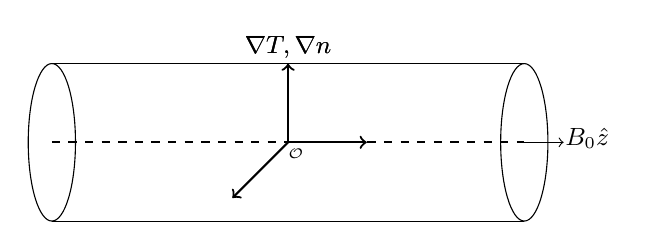
\begin{tikzpicture}[scale=1]
			% Cylinder axis from left to right
			(0,0) ellipse (0.3 and 1) % left cap
			(6,0) ellipse (0.3 and 1); % right cap (hidden)
			% Body
			(0,1) -- (6,1) arc (90:-90:1 and 0.3) -- (0,-1) arc (-90:90:1 and 0.3);
			% Front and back ellipses
			\draw (0,0) ellipse (0.3 and 1);
			\draw (6,0) ellipse (0.3 and 1);
			\foreach \angle in {0,90, 225}{
				\draw[->,thick] (3,0) -- ++(\angle:1);
			}\foreach \angle in {0,90}{
				\node at (3,1.2) {\small{$\nabla T, \nabla n$}} ++(\angle:1);
			}
			\node at (3.1,-0.15) {\tiny{$\mathcal{O}$}};
			% Cylinder outline
			\draw (0,1) -- (6,1);
			\draw (0,-1) -- (6,-1);
			\draw[dashed, thick] (0.0,0.0) -- (6.0,0.0);
			\draw[->] (6.0,0.0) -- (6.5,0.0);
			\node at (6.8,0.05) {\small{$B_0\hat{z}$}};
		\end{tikzpicture}
		\caption{Plasma Cil\'indrico con campo uniforme y transporte radial de part\'iculas y energ\'ia}
	\end{figure}

  Sin embargo, la geometr\'ia que usualmente queremos trabajar es una toroidal ya sea para un Tokamak o un Stellerator. Desde un punto de vista topol\'ogico simplemente podemos doblar el cil\'indro sobre si mismo y obtendremos la geometr\'ia deseada (ve\'ase la Figura \ref{fig:tor}), sin embargo, esto tiene implicaciones sobre el campo magn\'etico y el transporte en el plasma, tambi\'en sobre el confinamiento. En resumen, la complejidad del problema supera por mucho las consideraciones que hemos hecho hasta el momento. Sin embargo, parte del pr\'oposito de este trabajo es ver que tanto difieren los resultados y bajo que r\'egimenes la aproximaci\'on es est\'a dentro de la tolerancia y permite explicar, al menos de forma cualitativa el comportamiento de la densidad y la temperatura del plasma. 

  \begin{figure}[htb!]
    \centering
  	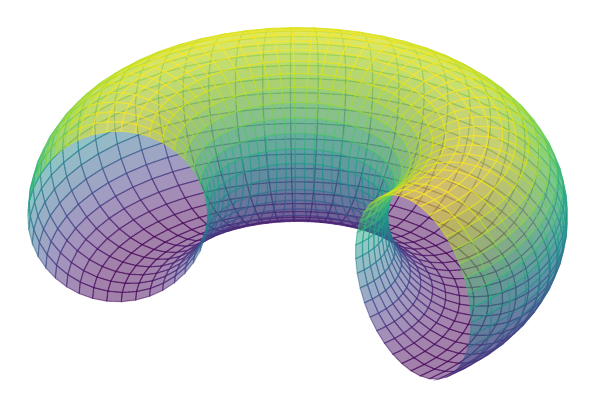
\begin{tikzpicture}
		\begin{axis}[
			view={180}{50}, % Viewing angle
			hide axis, % Hide the axes
			samples=40, % Number of samples in the x direction
			samples y=40, % Number of samples in the y direction
			domain=0:360,
			y domain=130:360,
			z buffer=sort, % Improve 3D rendering
			colormap name=viridis
			]
			\addplot3[
			thin,
			surf,
			shader=flat,
			opacity=0.5, % Add some transparency
			mesh/rows=40, % Match the number of samples
			mesh/cols=40 % Match the number of samples y
			]
			(
			{(2 + cos(x)) * cos(y)}, 
			{(2 + cos(x)) * sin(y)}, 
			{sin(x)}
			);
		\end{axis}
	\end{tikzpicture}
    \caption{Geometr\'ia toroidal de los dispositivos de confinamiento de plasma que se puede ver como el doblamiento del cil\'indro.}
    \label{fig:tor}
  \end{figure}

Se pueden ver que finalmente las relaciones de transporte radial, o flujo de part\'iculas y energ\'ia se pueden escribir como

  \begin{eqnarray}
    \Gamma_n &=& -A\left<\textbf{D}\cdot\nabla n\right>_{\partial V} \label{eq:partflux}\\
    \Gamma_E &=& -A\left<\pmb{\chi}\cdot\nabla T\right>_{\partial V} + \frac{3}{2}A\left<T\pmb{\Gamma}\right>_{\partial V}\label{eq:energyflux}
    \end{eqnarray}
    
  Las cantidades $\chi$ y $D$ deben ser estudiadas m\'as a fondo antes de asumir que son simplemente coeficientes, ya que podr\'an depender de la densidad $n$ y la temperatura $T$.
